\documentclass[twoside]{book}

% Packages required by doxygen
\usepackage{fixltx2e}
\usepackage{calc}
\usepackage{doxygen}
\usepackage[export]{adjustbox} % also loads graphicx
\usepackage{graphicx}
\usepackage[utf8]{inputenc}
\usepackage{makeidx}
\usepackage{multicol}
\usepackage{multirow}
\PassOptionsToPackage{warn}{textcomp}
\usepackage{textcomp}
\usepackage[nointegrals]{wasysym}
\usepackage[table]{xcolor}

% Font selection
\usepackage[T1]{fontenc}
\usepackage[scaled=.90]{helvet}
\usepackage{courier}
\usepackage{amssymb}
\usepackage{sectsty}
\renewcommand{\familydefault}{\sfdefault}
\allsectionsfont{%
  \fontseries{bc}\selectfont%
  \color{darkgray}%
}
\renewcommand{\DoxyLabelFont}{%
  \fontseries{bc}\selectfont%
  \color{darkgray}%
}
\newcommand{\+}{\discretionary{\mbox{\scriptsize$\hookleftarrow$}}{}{}}

% Page & text layout
\usepackage{geometry}
\geometry{%
  a4paper,%
  top=2.5cm,%
  bottom=2.5cm,%
  left=2.5cm,%
  right=2.5cm%
}
\tolerance=750
\hfuzz=15pt
\hbadness=750
\setlength{\emergencystretch}{15pt}
\setlength{\parindent}{0cm}
\setlength{\parskip}{3ex plus 2ex minus 2ex}
\makeatletter
\renewcommand{\paragraph}{%
  \@startsection{paragraph}{4}{0ex}{-1.0ex}{1.0ex}{%
    \normalfont\normalsize\bfseries\SS@parafont%
  }%
}
\renewcommand{\subparagraph}{%
  \@startsection{subparagraph}{5}{0ex}{-1.0ex}{1.0ex}{%
    \normalfont\normalsize\bfseries\SS@subparafont%
  }%
}
\makeatother

% Headers & footers
\usepackage{fancyhdr}
\pagestyle{fancyplain}
\fancyhead[LE]{\fancyplain{}{\bfseries\thepage}}
\fancyhead[CE]{\fancyplain{}{}}
\fancyhead[RE]{\fancyplain{}{\bfseries\leftmark}}
\fancyhead[LO]{\fancyplain{}{\bfseries\rightmark}}
\fancyhead[CO]{\fancyplain{}{}}
\fancyhead[RO]{\fancyplain{}{\bfseries\thepage}}
\fancyfoot[LE]{\fancyplain{}{}}
\fancyfoot[CE]{\fancyplain{}{}}
\fancyfoot[RE]{\fancyplain{}{\bfseries\scriptsize Generated by Doxygen }}
\fancyfoot[LO]{\fancyplain{}{\bfseries\scriptsize Generated by Doxygen }}
\fancyfoot[CO]{\fancyplain{}{}}
\fancyfoot[RO]{\fancyplain{}{}}
\renewcommand{\footrulewidth}{0.4pt}
\renewcommand{\chaptermark}[1]{%
  \markboth{#1}{}%
}
\renewcommand{\sectionmark}[1]{%
  \markright{\thesection\ #1}%
}

% Indices & bibliography
\usepackage{natbib}
\usepackage[titles]{tocloft}
\setcounter{tocdepth}{3}
\setcounter{secnumdepth}{5}
\makeindex

% Hyperlinks (required, but should be loaded last)
\usepackage{ifpdf}
\ifpdf
  \usepackage[pdftex,pagebackref=true]{hyperref}
\else
  \usepackage[ps2pdf,pagebackref=true]{hyperref}
\fi
\hypersetup{%
  colorlinks=true,%
  linkcolor=blue,%
  citecolor=blue,%
  unicode%
}

% Custom commands
\newcommand{\clearemptydoublepage}{%
  \newpage{\pagestyle{empty}\cleardoublepage}%
}

\usepackage{caption}
\captionsetup{labelsep=space,justification=centering,font={bf},singlelinecheck=off,skip=4pt,position=top}

%===== C O N T E N T S =====

\begin{document}

% Titlepage & ToC
\hypersetup{pageanchor=false,
             bookmarksnumbered=true,
             pdfencoding=unicode
            }
\pagenumbering{alph}
\begin{titlepage}
\vspace*{7cm}
\begin{center}%
{\Large Ackermann\+\_\+\+Steering\+\_\+\+Control\+\_\+\+M\+T15 }\\
\vspace*{1cm}
{\large Generated by Doxygen 1.8.13}\\
\end{center}
\end{titlepage}
\clearemptydoublepage
\pagenumbering{roman}
\tableofcontents
\clearemptydoublepage
\pagenumbering{arabic}
\hypersetup{pageanchor=true}

%--- Begin generated contents ---
\chapter{Class Index}
\section{Class List}
Here are the classes, structs, unions and interfaces with brief descriptions\+:\begin{DoxyCompactList}
\item\contentsline{section}{\hyperlink{classController}{Controller} \\*Class to hold goal attributes and members }{\pageref{classController}}{}
\item\contentsline{section}{\hyperlink{classConvergence}{Convergence} \\*Class to visualize \hyperlink{classConvergence}{Convergence} }{\pageref{classConvergence}}{}
\item\contentsline{section}{\hyperlink{classForwardKinematics}{Forward\+Kinematics} \\*Class to apply forward kinematics }{\pageref{classForwardKinematics}}{}
\item\contentsline{section}{\hyperlink{classInverseKinematics}{Inverse\+Kinematics} \\*Class to apply inverse kinematics }{\pageref{classInverseKinematics}}{}
\item\contentsline{section}{\hyperlink{classPID}{P\+ID} \\*Class to hold \hyperlink{classPID}{P\+ID} \hyperlink{classController}{Controller} attributes and members }{\pageref{classPID}}{}
\item\contentsline{section}{\hyperlink{classRobot}{Robot} \\*Class to hold robot\textquotesingle{}s attributes and members }{\pageref{classRobot}}{}
\item\contentsline{section}{\hyperlink{classSensor}{Sensor} \\*Class to hold current state of robot }{\pageref{classSensor}}{}
\end{DoxyCompactList}

\chapter{Class Documentation}
\hypertarget{classController}{}\section{Controller Class Reference}
\label{classController}\index{Controller@{Controller}}


Class to hold goal attributes and members.  




{\ttfamily \#include $<$controller.\+hpp$>$}

\subsection*{Public Member Functions}
\begin{DoxyCompactItemize}
\item 
\mbox{\Hypertarget{classController_a95c56822d667e94b031451729ce069a9}\label{classController_a95c56822d667e94b031451729ce069a9}} 
\hyperlink{classController_a95c56822d667e94b031451729ce069a9}{Controller} ()
\begin{DoxyCompactList}\small\item\em Constrctor of Class \hyperlink{classController}{Controller} to initialize goal values. \end{DoxyCompactList}\item 
\mbox{\Hypertarget{classController_a0ab87934c4f7a266cfdb86e0f36bc1b5}\label{classController_a0ab87934c4f7a266cfdb86e0f36bc1b5}} 
\hyperlink{classController_a0ab87934c4f7a266cfdb86e0f36bc1b5}{$\sim$\+Controller} ()
\begin{DoxyCompactList}\small\item\em Destructor of class \hyperlink{classController}{Controller}. \end{DoxyCompactList}\item 
double \hyperlink{classController_ac0aa43a79fdc74c7bd75bf383c5b80e0}{get\+Goal\+Heading} ()
\begin{DoxyCompactList}\small\item\em Get goal heading value. (0 to 3.\+14 radians) \end{DoxyCompactList}\item 
double \hyperlink{classController_ab8161275786c47cc70d1ad82f3c476e2}{get\+Goal\+Speed} ()
\begin{DoxyCompactList}\small\item\em Get goal speed value. (in meters/seconds) \end{DoxyCompactList}\item 
void \hyperlink{classController_ad41ca82c11e43a21d32c23ad159e747b}{set\+Goal} (double goal\+\_\+heading, double goal\+\_\+speed)
\begin{DoxyCompactList}\small\item\em Get set goal heading and speed values. \end{DoxyCompactList}\end{DoxyCompactItemize}


\subsection{Detailed Description}
Class to hold goal attributes and members. 

Definition at line 40 of file controller.\+hpp.



\subsection{Member Function Documentation}
\mbox{\Hypertarget{classController_ac0aa43a79fdc74c7bd75bf383c5b80e0}\label{classController_ac0aa43a79fdc74c7bd75bf383c5b80e0}} 
\index{Controller@{Controller}!get\+Goal\+Heading@{get\+Goal\+Heading}}
\index{get\+Goal\+Heading@{get\+Goal\+Heading}!Controller@{Controller}}
\subsubsection{\texorpdfstring{get\+Goal\+Heading()}{getGoalHeading()}}
{\footnotesize\ttfamily double Controller\+::get\+Goal\+Heading (\begin{DoxyParamCaption}{ }\end{DoxyParamCaption})}



Get goal heading value. (0 to 3.\+14 radians) 


\begin{DoxyParams}{Parameters}
{\em void} & \\
\hline
\end{DoxyParams}
\begin{DoxyReturn}{Returns}
double -\/ \hyperlink{classRobot}{Robot}\textquotesingle{}s goal heading (in radians) 
\end{DoxyReturn}
Here is the caller graph for this function\+:
\nopagebreak
\begin{figure}[H]
\begin{center}
\leavevmode
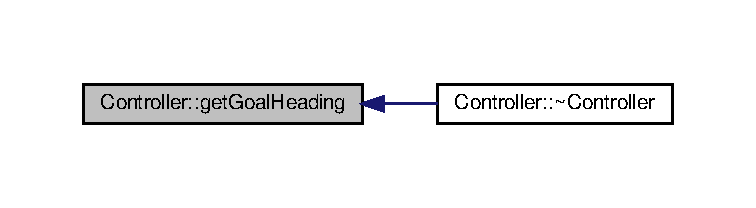
\includegraphics[width=350pt]{classController_ac0aa43a79fdc74c7bd75bf383c5b80e0_icgraph}
\end{center}
\end{figure}
\mbox{\Hypertarget{classController_ab8161275786c47cc70d1ad82f3c476e2}\label{classController_ab8161275786c47cc70d1ad82f3c476e2}} 
\index{Controller@{Controller}!get\+Goal\+Speed@{get\+Goal\+Speed}}
\index{get\+Goal\+Speed@{get\+Goal\+Speed}!Controller@{Controller}}
\subsubsection{\texorpdfstring{get\+Goal\+Speed()}{getGoalSpeed()}}
{\footnotesize\ttfamily double Controller\+::get\+Goal\+Speed (\begin{DoxyParamCaption}{ }\end{DoxyParamCaption})}



Get goal speed value. (in meters/seconds) 

\begin{DoxyReturn}{Returns}
double -\/ \hyperlink{classRobot}{Robot}\textquotesingle{}s goal speed (in meters/seconds) 
\end{DoxyReturn}
Here is the caller graph for this function\+:
\nopagebreak
\begin{figure}[H]
\begin{center}
\leavevmode
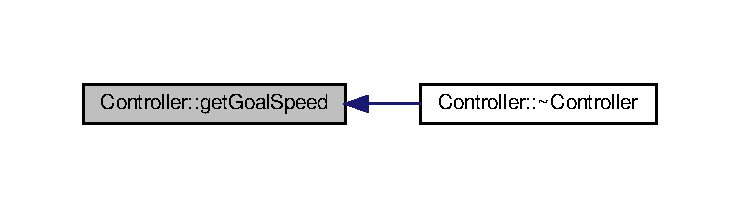
\includegraphics[width=350pt]{classController_ab8161275786c47cc70d1ad82f3c476e2_icgraph}
\end{center}
\end{figure}
\mbox{\Hypertarget{classController_ad41ca82c11e43a21d32c23ad159e747b}\label{classController_ad41ca82c11e43a21d32c23ad159e747b}} 
\index{Controller@{Controller}!set\+Goal@{set\+Goal}}
\index{set\+Goal@{set\+Goal}!Controller@{Controller}}
\subsubsection{\texorpdfstring{set\+Goal()}{setGoal()}}
{\footnotesize\ttfamily void Controller\+::set\+Goal (\begin{DoxyParamCaption}\item[{double}]{goal\+\_\+heading,  }\item[{double}]{goal\+\_\+speed }\end{DoxyParamCaption})}



Get set goal heading and speed values. 


\begin{DoxyParams}{Parameters}
{\em goal\+\_\+heading} & (0 to 3.\+14 radians) \\
\hline
{\em goal\+\_\+speed} & (in meters/seconds) \\
\hline
\end{DoxyParams}
\begin{DoxyReturn}{Returns}
void 
\end{DoxyReturn}
Here is the caller graph for this function\+:
\nopagebreak
\begin{figure}[H]
\begin{center}
\leavevmode
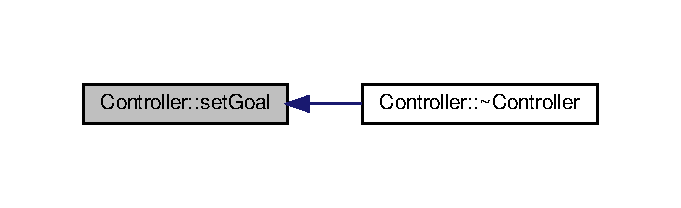
\includegraphics[width=327pt]{classController_ad41ca82c11e43a21d32c23ad159e747b_icgraph}
\end{center}
\end{figure}


The documentation for this class was generated from the following file\+:\begin{DoxyCompactItemize}
\item 
/home/maitreya/valgrind\+\_\+ws/\+Ackermann\+\_\+\+Steering\+\_\+\+Control/include/controller.\+hpp\end{DoxyCompactItemize}

\hypertarget{classConvergence}{}\section{Convergence Class Reference}
\label{classConvergence}\index{Convergence@{Convergence}}


Class to visualize \hyperlink{classConvergence}{Convergence}.  




{\ttfamily \#include $<$convergence.\+hpp$>$}

\subsection*{Public Member Functions}
\begin{DoxyCompactItemize}
\item 
\mbox{\Hypertarget{classConvergence_a644fb586d68b13c52f88379ad2122a8f}\label{classConvergence_a644fb586d68b13c52f88379ad2122a8f}} 
\hyperlink{classConvergence_a644fb586d68b13c52f88379ad2122a8f}{Convergence} ()
\begin{DoxyCompactList}\small\item\em Constructor for class \hyperlink{classConvergence}{Convergence}. \end{DoxyCompactList}\item 
\mbox{\Hypertarget{classConvergence_ab1b92e86a86f779f0b7ff9964f02030a}\label{classConvergence_ab1b92e86a86f779f0b7ff9964f02030a}} 
\hyperlink{classConvergence_ab1b92e86a86f779f0b7ff9964f02030a}{$\sim$\+Convergence} ()
\begin{DoxyCompactList}\small\item\em Destructor for class \hyperlink{classConvergence}{Convergence}. \end{DoxyCompactList}\item 
int \hyperlink{classConvergence_a7683c2efed8e5526481d361cb28bb6cf}{plot\+Convergence} (double, std\+::vector$<$ double $>$ \&, std\+::string \&)
\begin{DoxyCompactList}\small\item\em plot convergence of robot\textquotesingle{}s heading and speed \end{DoxyCompactList}\end{DoxyCompactItemize}


\subsection{Detailed Description}
Class to visualize \hyperlink{classConvergence}{Convergence}. 

Definition at line 43 of file convergence.\+hpp.



\subsection{Member Function Documentation}
\mbox{\Hypertarget{classConvergence_a7683c2efed8e5526481d361cb28bb6cf}\label{classConvergence_a7683c2efed8e5526481d361cb28bb6cf}} 
\index{Convergence@{Convergence}!plot\+Convergence@{plot\+Convergence}}
\index{plot\+Convergence@{plot\+Convergence}!Convergence@{Convergence}}
\subsubsection{\texorpdfstring{plot\+Convergence()}{plotConvergence()}}
{\footnotesize\ttfamily int Convergence\+::plot\+Convergence (\begin{DoxyParamCaption}\item[{double}]{,  }\item[{std\+::vector$<$ double $>$ \&}]{,  }\item[{std\+::string \&}]{ }\end{DoxyParamCaption})}



plot convergence of robot\textquotesingle{}s heading and speed 


\begin{DoxyParams}{Parameters}
{\em double} & -\/ speed output from fk \\
\hline
\end{DoxyParams}
\begin{DoxyReturn}{Returns}
void 
\end{DoxyReturn}
Here is the caller graph for this function\+:
\nopagebreak
\begin{figure}[H]
\begin{center}
\leavevmode
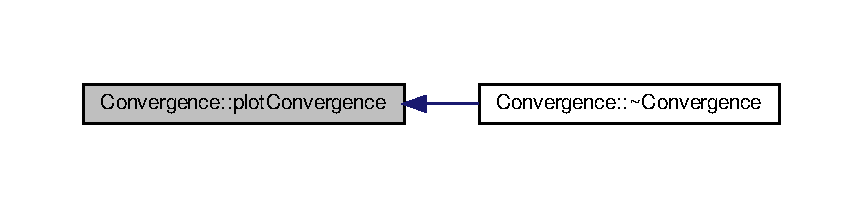
\includegraphics[width=350pt]{classConvergence_a7683c2efed8e5526481d361cb28bb6cf_icgraph}
\end{center}
\end{figure}


The documentation for this class was generated from the following file\+:\begin{DoxyCompactItemize}
\item 
/home/maitreya/valgrind\+\_\+ws/\+Ackermann\+\_\+\+Steering\+\_\+\+Control/include/convergence.\+hpp\end{DoxyCompactItemize}

\hypertarget{classForwardKinematics}{}\section{Forward\+Kinematics Class Reference}
\label{classForwardKinematics}\index{Forward\+Kinematics@{Forward\+Kinematics}}


Class to apply forward kinematics.  




{\ttfamily \#include $<$forward\+\_\+kinematics.\+hpp$>$}

\subsection*{Public Member Functions}
\begin{DoxyCompactItemize}
\item 
\hyperlink{classForwardKinematics_aff7ff4cb9cf2c523b111f2c5f2ec5cc8}{Forward\+Kinematics} ()
\begin{DoxyCompactList}\small\item\em Consructor for class \hyperlink{classForwardKinematics}{Forward\+Kinematics} to initialize values local variables to 0. \end{DoxyCompactList}\item 
\mbox{\Hypertarget{classForwardKinematics_a78e9a1bc65b4262f88f0f1f60f2b6368}\label{classForwardKinematics_a78e9a1bc65b4262f88f0f1f60f2b6368}} 
\hyperlink{classForwardKinematics_a78e9a1bc65b4262f88f0f1f60f2b6368}{$\sim$\+Forward\+Kinematics} ()
\begin{DoxyCompactList}\small\item\em Destructor for class \hyperlink{classForwardKinematics}{Forward\+Kinematics}. \end{DoxyCompactList}\item 
double \hyperlink{classForwardKinematics_a6fdaaf30015b1628efed2407ea13c780}{get\+R1} ()
\begin{DoxyCompactList}\small\item\em Get turning raduis from centre of rear axle. (in meters) \end{DoxyCompactList}\item 
void \hyperlink{classForwardKinematics_ad4093b156610a520068844c7018a256e}{set\+D\+Theta} (double d\+\_\+theta)
\begin{DoxyCompactList}\small\item\em Set change in robot heading. (in radians) \end{DoxyCompactList}\item 
double \hyperlink{classForwardKinematics_a005d9cbb53f4dbb79b16defb52a8e76a}{calculate\+New\+Heading} (double goal\+\_\+heading)
\begin{DoxyCompactList}\small\item\em Calculate new heading required to reach the goal heading. (in radians) \end{DoxyCompactList}\item 
double \hyperlink{classForwardKinematics_af945b5d3d508aba54ea902674a65373c}{calculate\+New\+Speed} (double goal\+\_\+speed)
\begin{DoxyCompactList}\small\item\em Calculate new speed required to reach the goal speed. (in meters/seconds) \end{DoxyCompactList}\item 
bool \hyperlink{classForwardKinematics_ab5b26d5bc5c63148a7efa8361a851066}{goal\+Reached} (double goal\+\_\+heading, double goal\+\_\+speed)
\begin{DoxyCompactList}\small\item\em Boolean value for goal reached (True/\+False) \end{DoxyCompactList}\end{DoxyCompactItemize}
\subsection*{Public Attributes}
\begin{DoxyCompactItemize}
\item 
\mbox{\Hypertarget{classForwardKinematics_a7383b93f21d29c6a3db88533a809f28c}\label{classForwardKinematics_a7383b93f21d29c6a3db88533a809f28c}} 
std\+::vector$<$ double $>$ {\bfseries heading\+\_\+vector}
\item 
\mbox{\Hypertarget{classForwardKinematics_a8dd3201e71a1139616fb6ce329cd7df7}\label{classForwardKinematics_a8dd3201e71a1139616fb6ce329cd7df7}} 
std\+::vector$<$ double $>$ {\bfseries speed\+\_\+vector}
\end{DoxyCompactItemize}


\subsection{Detailed Description}
Class to apply forward kinematics. 

Definition at line 40 of file forward\+\_\+kinematics.\+hpp.



\subsection{Constructor \& Destructor Documentation}
\mbox{\Hypertarget{classForwardKinematics_aff7ff4cb9cf2c523b111f2c5f2ec5cc8}\label{classForwardKinematics_aff7ff4cb9cf2c523b111f2c5f2ec5cc8}} 
\index{Forward\+Kinematics@{Forward\+Kinematics}!Forward\+Kinematics@{Forward\+Kinematics}}
\index{Forward\+Kinematics@{Forward\+Kinematics}!Forward\+Kinematics@{Forward\+Kinematics}}
\subsubsection{\texorpdfstring{Forward\+Kinematics()}{ForwardKinematics()}}
{\footnotesize\ttfamily Forward\+Kinematics\+::\+Forward\+Kinematics (\begin{DoxyParamCaption}{ }\end{DoxyParamCaption})\hspace{0.3cm}{\ttfamily [inline]}}



Consructor for class \hyperlink{classForwardKinematics}{Forward\+Kinematics} to initialize values local variables to 0. 


\begin{DoxyParams}{Parameters}
{\em void} & \\
\hline
\end{DoxyParams}
\begin{DoxyReturn}{Returns}
void 
\end{DoxyReturn}


Definition at line 50 of file forward\+\_\+kinematics.\+hpp.



\subsection{Member Function Documentation}
\mbox{\Hypertarget{classForwardKinematics_a005d9cbb53f4dbb79b16defb52a8e76a}\label{classForwardKinematics_a005d9cbb53f4dbb79b16defb52a8e76a}} 
\index{Forward\+Kinematics@{Forward\+Kinematics}!calculate\+New\+Heading@{calculate\+New\+Heading}}
\index{calculate\+New\+Heading@{calculate\+New\+Heading}!Forward\+Kinematics@{Forward\+Kinematics}}
\subsubsection{\texorpdfstring{calculate\+New\+Heading()}{calculateNewHeading()}}
{\footnotesize\ttfamily double Forward\+Kinematics\+::calculate\+New\+Heading (\begin{DoxyParamCaption}\item[{double}]{goal\+\_\+heading }\end{DoxyParamCaption})}



Calculate new heading required to reach the goal heading. (in radians) 


\begin{DoxyParams}{Parameters}
{\em goal\+\_\+heading} & double -\/ robot\textquotesingle{}s goal heading \\
\hline
\end{DoxyParams}
\begin{DoxyReturn}{Returns}
double -\/ new heading required to reach the goal heading 
\end{DoxyReturn}
Here is the caller graph for this function\+:
\nopagebreak
\begin{figure}[H]
\begin{center}
\leavevmode
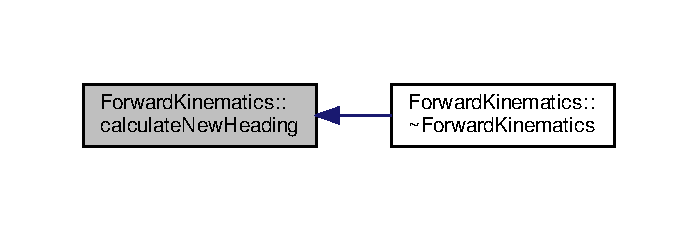
\includegraphics[width=335pt]{classForwardKinematics_a005d9cbb53f4dbb79b16defb52a8e76a_icgraph}
\end{center}
\end{figure}
\mbox{\Hypertarget{classForwardKinematics_af945b5d3d508aba54ea902674a65373c}\label{classForwardKinematics_af945b5d3d508aba54ea902674a65373c}} 
\index{Forward\+Kinematics@{Forward\+Kinematics}!calculate\+New\+Speed@{calculate\+New\+Speed}}
\index{calculate\+New\+Speed@{calculate\+New\+Speed}!Forward\+Kinematics@{Forward\+Kinematics}}
\subsubsection{\texorpdfstring{calculate\+New\+Speed()}{calculateNewSpeed()}}
{\footnotesize\ttfamily double Forward\+Kinematics\+::calculate\+New\+Speed (\begin{DoxyParamCaption}\item[{double}]{goal\+\_\+speed }\end{DoxyParamCaption})}



Calculate new speed required to reach the goal speed. (in meters/seconds) 


\begin{DoxyParams}{Parameters}
{\em goal\+\_\+speed} & double -\/ robot\textquotesingle{}s goal speed \\
\hline
\end{DoxyParams}
\begin{DoxyReturn}{Returns}
double -\/ new speed required to reach the goal speed 
\end{DoxyReturn}
Here is the caller graph for this function\+:
\nopagebreak
\begin{figure}[H]
\begin{center}
\leavevmode
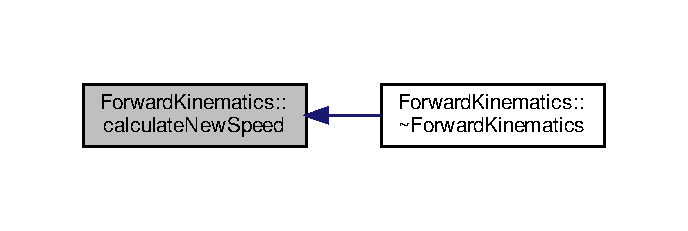
\includegraphics[width=330pt]{classForwardKinematics_af945b5d3d508aba54ea902674a65373c_icgraph}
\end{center}
\end{figure}
\mbox{\Hypertarget{classForwardKinematics_a6fdaaf30015b1628efed2407ea13c780}\label{classForwardKinematics_a6fdaaf30015b1628efed2407ea13c780}} 
\index{Forward\+Kinematics@{Forward\+Kinematics}!get\+R1@{get\+R1}}
\index{get\+R1@{get\+R1}!Forward\+Kinematics@{Forward\+Kinematics}}
\subsubsection{\texorpdfstring{get\+R1()}{getR1()}}
{\footnotesize\ttfamily double Forward\+Kinematics\+::get\+R1 (\begin{DoxyParamCaption}{ }\end{DoxyParamCaption})}



Get turning raduis from centre of rear axle. (in meters) 


\begin{DoxyParams}{Parameters}
{\em void} & \\
\hline
\end{DoxyParams}
\begin{DoxyReturn}{Returns}
double -\/ turning raduis from centre of rear axle (in meters) 
\end{DoxyReturn}
Here is the caller graph for this function\+:
\nopagebreak
\begin{figure}[H]
\begin{center}
\leavevmode
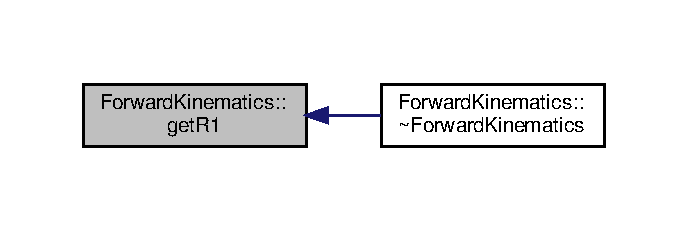
\includegraphics[width=330pt]{classForwardKinematics_a6fdaaf30015b1628efed2407ea13c780_icgraph}
\end{center}
\end{figure}
\mbox{\Hypertarget{classForwardKinematics_ab5b26d5bc5c63148a7efa8361a851066}\label{classForwardKinematics_ab5b26d5bc5c63148a7efa8361a851066}} 
\index{Forward\+Kinematics@{Forward\+Kinematics}!goal\+Reached@{goal\+Reached}}
\index{goal\+Reached@{goal\+Reached}!Forward\+Kinematics@{Forward\+Kinematics}}
\subsubsection{\texorpdfstring{goal\+Reached()}{goalReached()}}
{\footnotesize\ttfamily bool Forward\+Kinematics\+::goal\+Reached (\begin{DoxyParamCaption}\item[{double}]{goal\+\_\+heading,  }\item[{double}]{goal\+\_\+speed }\end{DoxyParamCaption})}



Boolean value for goal reached (True/\+False) 


\begin{DoxyParams}{Parameters}
{\em goal\+\_\+heading} & double -\/ robot\textquotesingle{}s goal heading \\
\hline
{\em goal\+\_\+speed} & double -\/ robot\textquotesingle{}s goal speed \\
\hline
\end{DoxyParams}
\begin{DoxyReturn}{Returns}
bool 
\end{DoxyReturn}
Here is the caller graph for this function\+:
\nopagebreak
\begin{figure}[H]
\begin{center}
\leavevmode
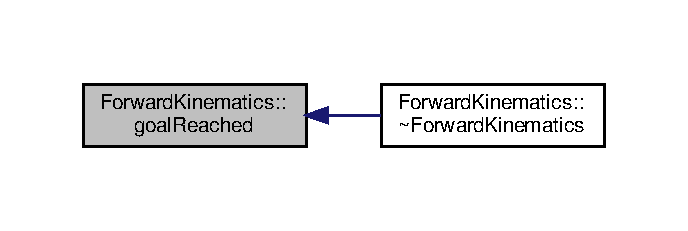
\includegraphics[width=330pt]{classForwardKinematics_ab5b26d5bc5c63148a7efa8361a851066_icgraph}
\end{center}
\end{figure}
\mbox{\Hypertarget{classForwardKinematics_ad4093b156610a520068844c7018a256e}\label{classForwardKinematics_ad4093b156610a520068844c7018a256e}} 
\index{Forward\+Kinematics@{Forward\+Kinematics}!set\+D\+Theta@{set\+D\+Theta}}
\index{set\+D\+Theta@{set\+D\+Theta}!Forward\+Kinematics@{Forward\+Kinematics}}
\subsubsection{\texorpdfstring{set\+D\+Theta()}{setDTheta()}}
{\footnotesize\ttfamily void Forward\+Kinematics\+::set\+D\+Theta (\begin{DoxyParamCaption}\item[{double}]{d\+\_\+theta }\end{DoxyParamCaption})}



Set change in robot heading. (in radians) 


\begin{DoxyParams}{Parameters}
{\em d\+\_\+theta} & double -\/ change in robot\textquotesingle{}s heading. (in radians) \\
\hline
\end{DoxyParams}
\begin{DoxyReturn}{Returns}
void 
\end{DoxyReturn}
Here is the caller graph for this function\+:
\nopagebreak
\begin{figure}[H]
\begin{center}
\leavevmode
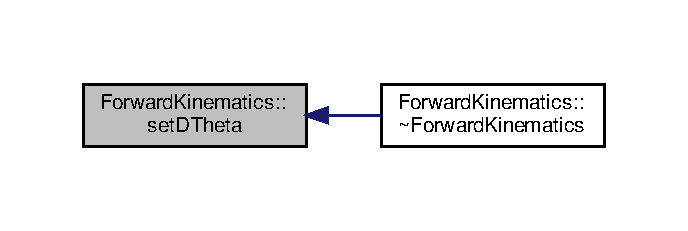
\includegraphics[width=330pt]{classForwardKinematics_ad4093b156610a520068844c7018a256e_icgraph}
\end{center}
\end{figure}


The documentation for this class was generated from the following file\+:\begin{DoxyCompactItemize}
\item 
/home/maitreya/valgrind\+\_\+ws/\+Ackermann\+\_\+\+Steering\+\_\+\+Control/include/forward\+\_\+kinematics.\+hpp\end{DoxyCompactItemize}

\hypertarget{classInverseKinematics}{}\section{Inverse\+Kinematics Class Reference}
\label{classInverseKinematics}\index{Inverse\+Kinematics@{Inverse\+Kinematics}}


Class to apply inverse kinematics.  




{\ttfamily \#include $<$inverse\+\_\+kinematics.\+hpp$>$}

\subsection*{Public Member Functions}
\begin{DoxyCompactItemize}
\item 
\mbox{\Hypertarget{classInverseKinematics_a5ac416b45f9039ce28836cd73193d04b}\label{classInverseKinematics_a5ac416b45f9039ce28836cd73193d04b}} 
\hyperlink{classInverseKinematics_a5ac416b45f9039ce28836cd73193d04b}{Inverse\+Kinematics} ()
\begin{DoxyCompactList}\small\item\em Constructor for class \hyperlink{classInverseKinematics}{Inverse\+Kinematics}. \end{DoxyCompactList}\item 
\mbox{\Hypertarget{classInverseKinematics_af82fba3aeac080112db67265438bf30c}\label{classInverseKinematics_af82fba3aeac080112db67265438bf30c}} 
\hyperlink{classInverseKinematics_af82fba3aeac080112db67265438bf30c}{$\sim$\+Inverse\+Kinematics} ()
\begin{DoxyCompactList}\small\item\em Destructor for class \hyperlink{classInverseKinematics}{Inverse\+Kinematics}. \end{DoxyCompactList}\item 
void \hyperlink{classInverseKinematics_a5b4820979ff3b4b6e0a3346cd472fefe}{calculate\+Wheel\+Angles} (double)
\begin{DoxyCompactList}\small\item\em Calculate the left and right wheel angles based on heading output of fk. (in radians) \end{DoxyCompactList}\item 
void \hyperlink{classInverseKinematics_a7e72ae559e17363495da967d98fb7985}{calculate\+Wheel\+Speeds} (double)
\begin{DoxyCompactList}\small\item\em Calculate the left and right wheel speeds based on heading output of fk. (in ratations/second) \end{DoxyCompactList}\end{DoxyCompactItemize}


\subsection{Detailed Description}
Class to apply inverse kinematics. 

Definition at line 40 of file inverse\+\_\+kinematics.\+hpp.



\subsection{Member Function Documentation}
\mbox{\Hypertarget{classInverseKinematics_a5b4820979ff3b4b6e0a3346cd472fefe}\label{classInverseKinematics_a5b4820979ff3b4b6e0a3346cd472fefe}} 
\index{Inverse\+Kinematics@{Inverse\+Kinematics}!calculate\+Wheel\+Angles@{calculate\+Wheel\+Angles}}
\index{calculate\+Wheel\+Angles@{calculate\+Wheel\+Angles}!Inverse\+Kinematics@{Inverse\+Kinematics}}
\subsubsection{\texorpdfstring{calculate\+Wheel\+Angles()}{calculateWheelAngles()}}
{\footnotesize\ttfamily void Inverse\+Kinematics\+::calculate\+Wheel\+Angles (\begin{DoxyParamCaption}\item[{double}]{ }\end{DoxyParamCaption})}



Calculate the left and right wheel angles based on heading output of fk. (in radians) 


\begin{DoxyParams}{Parameters}
{\em double} & -\/ heading output from fk (in radians) \\
\hline
\end{DoxyParams}
\begin{DoxyReturn}{Returns}
void 
\end{DoxyReturn}
Here is the caller graph for this function\+:
\nopagebreak
\begin{figure}[H]
\begin{center}
\leavevmode
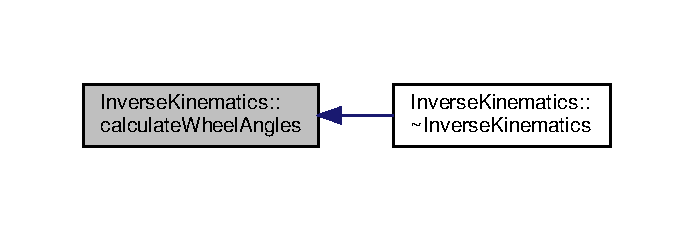
\includegraphics[width=333pt]{classInverseKinematics_a5b4820979ff3b4b6e0a3346cd472fefe_icgraph}
\end{center}
\end{figure}
\mbox{\Hypertarget{classInverseKinematics_a7e72ae559e17363495da967d98fb7985}\label{classInverseKinematics_a7e72ae559e17363495da967d98fb7985}} 
\index{Inverse\+Kinematics@{Inverse\+Kinematics}!calculate\+Wheel\+Speeds@{calculate\+Wheel\+Speeds}}
\index{calculate\+Wheel\+Speeds@{calculate\+Wheel\+Speeds}!Inverse\+Kinematics@{Inverse\+Kinematics}}
\subsubsection{\texorpdfstring{calculate\+Wheel\+Speeds()}{calculateWheelSpeeds()}}
{\footnotesize\ttfamily void Inverse\+Kinematics\+::calculate\+Wheel\+Speeds (\begin{DoxyParamCaption}\item[{double}]{ }\end{DoxyParamCaption})}



Calculate the left and right wheel speeds based on heading output of fk. (in ratations/second) 


\begin{DoxyParams}{Parameters}
{\em double} & -\/ speed output from fk (in meters/second) \\
\hline
\end{DoxyParams}
\begin{DoxyReturn}{Returns}
void 
\end{DoxyReturn}
Here is the caller graph for this function\+:
\nopagebreak
\begin{figure}[H]
\begin{center}
\leavevmode
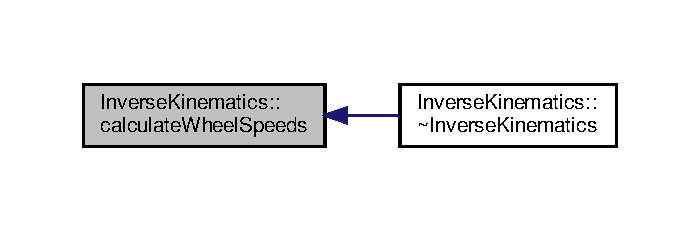
\includegraphics[width=336pt]{classInverseKinematics_a7e72ae559e17363495da967d98fb7985_icgraph}
\end{center}
\end{figure}


The documentation for this class was generated from the following file\+:\begin{DoxyCompactItemize}
\item 
/home/maitreya/valgrind\+\_\+ws/\+Ackermann\+\_\+\+Steering\+\_\+\+Control/include/inverse\+\_\+kinematics.\+hpp\end{DoxyCompactItemize}

\hypertarget{classPID}{}\section{P\+ID Class Reference}
\label{classPID}\index{P\+ID@{P\+ID}}


Class to hold \hyperlink{classPID}{P\+ID} \hyperlink{classController}{Controller} attributes and members.  




{\ttfamily \#include $<$pid.\+hpp$>$}

\subsection*{Public Member Functions}
\begin{DoxyCompactItemize}
\item 
\hyperlink{classPID_a74e83c18b71000d5e9d9ff4f0832045c}{P\+ID} (double Kp, double Ki, double Kd, double dt, double min, double max)
\begin{DoxyCompactList}\small\item\em Constructor for class \hyperlink{classPID}{P\+ID}. \end{DoxyCompactList}\item 
\mbox{\Hypertarget{classPID_ab7d389fc5b88d881bc25f5dafd360441}\label{classPID_ab7d389fc5b88d881bc25f5dafd360441}} 
\hyperlink{classPID_ab7d389fc5b88d881bc25f5dafd360441}{$\sim$\+P\+ID} ()
\begin{DoxyCompactList}\small\item\em Destructor for class \hyperlink{classPID}{P\+ID}. \end{DoxyCompactList}\item 
double \hyperlink{classPID_acb5ef99f0f57357393fd3556a413afe9}{compute} (double current\+\_\+value, double desired\+\_\+value)
\begin{DoxyCompactList}\small\item\em Calculate the output based on the current value and the desired value. \end{DoxyCompactList}\item 
double \hyperlink{classPID_a52625de61b1b2977b2c26ddb2698f14e}{get\+Kp} ()
\begin{DoxyCompactList}\small\item\em Get the Kp value. \end{DoxyCompactList}\item 
double \hyperlink{classPID_a89dedae29ef5a1359fd438824523bfc5}{get\+Ki} ()
\begin{DoxyCompactList}\small\item\em Get the Ki value. \end{DoxyCompactList}\item 
double \hyperlink{classPID_a39997546e8d1025c6c867e31e8b8e916}{get\+Kd} ()
\begin{DoxyCompactList}\small\item\em Get the Kd value. \end{DoxyCompactList}\item 
double \hyperlink{classPID_af8c9c5d64221b59cd56ac2543a33eb48}{get\+Dt} ()
\begin{DoxyCompactList}\small\item\em Get the dt. \end{DoxyCompactList}\end{DoxyCompactItemize}


\subsection{Detailed Description}
Class to hold \hyperlink{classPID}{P\+ID} \hyperlink{classController}{Controller} attributes and members. 

Definition at line 40 of file pid.\+hpp.



\subsection{Constructor \& Destructor Documentation}
\mbox{\Hypertarget{classPID_a74e83c18b71000d5e9d9ff4f0832045c}\label{classPID_a74e83c18b71000d5e9d9ff4f0832045c}} 
\index{P\+ID@{P\+ID}!P\+ID@{P\+ID}}
\index{P\+ID@{P\+ID}!P\+ID@{P\+ID}}
\subsubsection{\texorpdfstring{P\+I\+D()}{PID()}}
{\footnotesize\ttfamily P\+I\+D\+::\+P\+ID (\begin{DoxyParamCaption}\item[{double}]{Kp,  }\item[{double}]{Ki,  }\item[{double}]{Kd,  }\item[{double}]{dt,  }\item[{double}]{min,  }\item[{double}]{max }\end{DoxyParamCaption})\hspace{0.3cm}{\ttfamily [inline]}}



Constructor for class \hyperlink{classPID}{P\+ID}. 


\begin{DoxyParams}{Parameters}
{\em Kp} & double -\/ Proportional gain constant \\
\hline
{\em Ki} & double -\/ Integral gain constant \\
\hline
{\em Kd} & double -\/ Deravitive gain constant \\
\hline
{\em dt} & double -\/ Sampling time \\
\hline
{\em min} & double -\/ Minimum limit of output value \\
\hline
{\em max} & double -\/ Maximum limit of output value \\
\hline
\end{DoxyParams}


Definition at line 51 of file pid.\+hpp.



\subsection{Member Function Documentation}
\mbox{\Hypertarget{classPID_acb5ef99f0f57357393fd3556a413afe9}\label{classPID_acb5ef99f0f57357393fd3556a413afe9}} 
\index{P\+ID@{P\+ID}!compute@{compute}}
\index{compute@{compute}!P\+ID@{P\+ID}}
\subsubsection{\texorpdfstring{compute()}{compute()}}
{\footnotesize\ttfamily double P\+I\+D\+::compute (\begin{DoxyParamCaption}\item[{double}]{current\+\_\+value,  }\item[{double}]{desired\+\_\+value }\end{DoxyParamCaption})}



Calculate the output based on the current value and the desired value. 


\begin{DoxyParams}{Parameters}
{\em current\+\_\+value} & double -\/ current value of system \\
\hline
{\em desired\+\_\+value} & double -\/ desired value of system \\
\hline
\end{DoxyParams}
\begin{DoxyReturn}{Returns}
void 
\end{DoxyReturn}
Here is the caller graph for this function\+:
\nopagebreak
\begin{figure}[H]
\begin{center}
\leavevmode
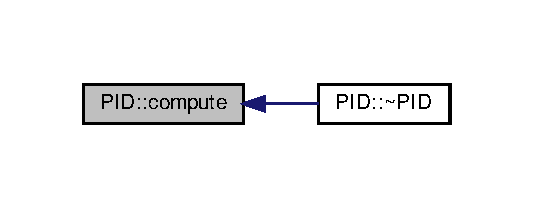
\includegraphics[width=256pt]{classPID_acb5ef99f0f57357393fd3556a413afe9_icgraph}
\end{center}
\end{figure}
\mbox{\Hypertarget{classPID_af8c9c5d64221b59cd56ac2543a33eb48}\label{classPID_af8c9c5d64221b59cd56ac2543a33eb48}} 
\index{P\+ID@{P\+ID}!get\+Dt@{get\+Dt}}
\index{get\+Dt@{get\+Dt}!P\+ID@{P\+ID}}
\subsubsection{\texorpdfstring{get\+Dt()}{getDt()}}
{\footnotesize\ttfamily double P\+I\+D\+::get\+Dt (\begin{DoxyParamCaption}{ }\end{DoxyParamCaption})}



Get the dt. 

\begin{DoxyReturn}{Returns}
double -\/ Sampling time 
\end{DoxyReturn}
Here is the caller graph for this function\+:
\nopagebreak
\begin{figure}[H]
\begin{center}
\leavevmode
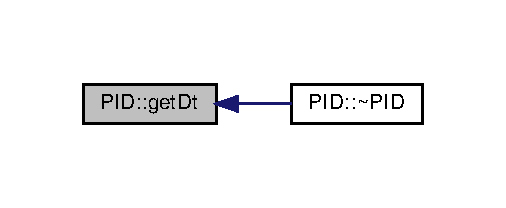
\includegraphics[width=243pt]{classPID_af8c9c5d64221b59cd56ac2543a33eb48_icgraph}
\end{center}
\end{figure}
\mbox{\Hypertarget{classPID_a39997546e8d1025c6c867e31e8b8e916}\label{classPID_a39997546e8d1025c6c867e31e8b8e916}} 
\index{P\+ID@{P\+ID}!get\+Kd@{get\+Kd}}
\index{get\+Kd@{get\+Kd}!P\+ID@{P\+ID}}
\subsubsection{\texorpdfstring{get\+Kd()}{getKd()}}
{\footnotesize\ttfamily double P\+I\+D\+::get\+Kd (\begin{DoxyParamCaption}{ }\end{DoxyParamCaption})}



Get the Kd value. 

\begin{DoxyReturn}{Returns}
double -\/ Value of Kd 
\end{DoxyReturn}
Here is the caller graph for this function\+:
\nopagebreak
\begin{figure}[H]
\begin{center}
\leavevmode
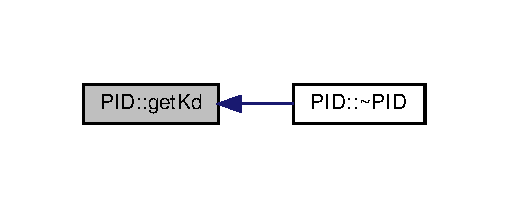
\includegraphics[width=244pt]{classPID_a39997546e8d1025c6c867e31e8b8e916_icgraph}
\end{center}
\end{figure}
\mbox{\Hypertarget{classPID_a89dedae29ef5a1359fd438824523bfc5}\label{classPID_a89dedae29ef5a1359fd438824523bfc5}} 
\index{P\+ID@{P\+ID}!get\+Ki@{get\+Ki}}
\index{get\+Ki@{get\+Ki}!P\+ID@{P\+ID}}
\subsubsection{\texorpdfstring{get\+Ki()}{getKi()}}
{\footnotesize\ttfamily double P\+I\+D\+::get\+Ki (\begin{DoxyParamCaption}{ }\end{DoxyParamCaption})}



Get the Ki value. 

\begin{DoxyReturn}{Returns}
double -\/ Value of Ki 
\end{DoxyReturn}
Here is the caller graph for this function\+:
\nopagebreak
\begin{figure}[H]
\begin{center}
\leavevmode
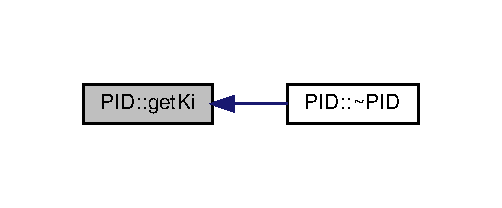
\includegraphics[width=241pt]{classPID_a89dedae29ef5a1359fd438824523bfc5_icgraph}
\end{center}
\end{figure}
\mbox{\Hypertarget{classPID_a52625de61b1b2977b2c26ddb2698f14e}\label{classPID_a52625de61b1b2977b2c26ddb2698f14e}} 
\index{P\+ID@{P\+ID}!get\+Kp@{get\+Kp}}
\index{get\+Kp@{get\+Kp}!P\+ID@{P\+ID}}
\subsubsection{\texorpdfstring{get\+Kp()}{getKp()}}
{\footnotesize\ttfamily double P\+I\+D\+::get\+Kp (\begin{DoxyParamCaption}{ }\end{DoxyParamCaption})}



Get the Kp value. 

\begin{DoxyReturn}{Returns}
double -\/ Value of Kp 
\end{DoxyReturn}
Here is the caller graph for this function\+:
\nopagebreak
\begin{figure}[H]
\begin{center}
\leavevmode
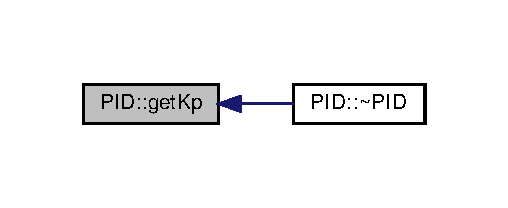
\includegraphics[width=244pt]{classPID_a52625de61b1b2977b2c26ddb2698f14e_icgraph}
\end{center}
\end{figure}


The documentation for this class was generated from the following file\+:\begin{DoxyCompactItemize}
\item 
/home/maitreya/valgrind\+\_\+ws/\+Ackermann\+\_\+\+Steering\+\_\+\+Control/include/pid.\+hpp\end{DoxyCompactItemize}

\hypertarget{classRobot}{}\section{Robot Class Reference}
\label{classRobot}\index{Robot@{Robot}}


Class to hold robot\textquotesingle{}s attributes and members.  




{\ttfamily \#include $<$robot.\+hpp$>$}

\subsection*{Public Member Functions}
\begin{DoxyCompactItemize}
\item 
\hyperlink{classRobot_a56b15a9c98244188ed610f62569a0aa0}{Robot} (double wheel\+\_\+base, double track\+\_\+width, double wheel\+\_\+radius, double left\+\_\+wheel\+\_\+vel, double right\+\_\+wheel\+\_\+vel, double left\+\_\+wheel\+\_\+ang, double right\+\_\+wheel\+\_\+ang, double com\+\_\+offset, double max\+\_\+steer\+\_\+angle)
\begin{DoxyCompactList}\small\item\em Constructor for class \hyperlink{classRobot}{Robot}. \end{DoxyCompactList}\item 
\mbox{\Hypertarget{classRobot_a924320124b09c2f2ac1621aa210d5f38}\label{classRobot_a924320124b09c2f2ac1621aa210d5f38}} 
\hyperlink{classRobot_a924320124b09c2f2ac1621aa210d5f38}{$\sim$\+Robot} ()
\begin{DoxyCompactList}\small\item\em Destructor for class \hyperlink{classRobot}{Robot}. \end{DoxyCompactList}\item 
double \hyperlink{classRobot_a31e2ab259ea221e1143141ee7765a8e2}{get\+Wheel\+Base} ()
\begin{DoxyCompactList}\small\item\em Get wheelbase of robot. (in meters) \end{DoxyCompactList}\item 
double \hyperlink{classRobot_a4a8df828fb337ab4505f3513bd46f410}{get\+Track\+Width} ()
\begin{DoxyCompactList}\small\item\em Get track width of robot. (in meters) \end{DoxyCompactList}\item 
double \hyperlink{classRobot_a419b324c8db1f6e7e1dd65b5a15f3049}{get\+Wheel\+Radius} ()
\begin{DoxyCompactList}\small\item\em Get wheel radius of robot. (in meters) \end{DoxyCompactList}\item 
double \hyperlink{classRobot_a99559e14e93539d1deaf5f0405dfce76}{get\+Left\+Wheel\+Vel} ()
\begin{DoxyCompactList}\small\item\em Get left drive wheel speed of robot. (in rotations/second) \end{DoxyCompactList}\item 
double \hyperlink{classRobot_a4596767fd5ee2f6a923523a298d584fb}{get\+Right\+Wheel\+Vel} ()
\begin{DoxyCompactList}\small\item\em Get right drive wheel speed of robot. (in rotations/second) \end{DoxyCompactList}\item 
double \hyperlink{classRobot_a3e230967bf4b167aaa20d442c6c5ceb0}{get\+Left\+Wheel\+Ang} ()
\begin{DoxyCompactList}\small\item\em Get left steering wheel angle of robot. (in radians) \end{DoxyCompactList}\item 
double \hyperlink{classRobot_aaa3dd6bad00b406b62bb58af2dd37ca4}{get\+Right\+Wheel\+Ang} ()
\begin{DoxyCompactList}\small\item\em Get right steering wheel angle of robot. (in radians) \end{DoxyCompactList}\item 
double \hyperlink{classRobot_a7ec7471708cfb59d26baefda819fa26b}{get\+Com\+Offset} ()
\begin{DoxyCompactList}\small\item\em Get Offset of robot\textquotesingle{}s centre of mass from centre of rear axle. (in meters) \end{DoxyCompactList}\item 
double \hyperlink{classRobot_ad51f91ba00dfe4efa1bf0a10ea3213e6}{get\+Max\+Steer\+Angle} ()
\begin{DoxyCompactList}\small\item\em Get maximum steering angle of robot. (in radians) \end{DoxyCompactList}\item 
void \hyperlink{classRobot_ab86642effe20a530827e4c2fc457ddb4}{set\+Left\+Wheel\+Vel} (double)
\begin{DoxyCompactList}\small\item\em Set left drive wheel speed of robot. \end{DoxyCompactList}\item 
void \hyperlink{classRobot_a89e3ada15839330f45c350b67ba746f3}{set\+Right\+Wheel\+Vel} (double)
\begin{DoxyCompactList}\small\item\em Set right drive wheel speed of robot. \end{DoxyCompactList}\item 
void \hyperlink{classRobot_adbe4d758d302d3fa70fedf5af9c82afc}{set\+Left\+Wheel\+Ang} (double)
\begin{DoxyCompactList}\small\item\em Set left drive wheel angle of robot. (in rotations/second) \end{DoxyCompactList}\item 
void \hyperlink{classRobot_a3d7a12ec4cd50436d46363de93a4f9b2}{set\+Right\+Wheel\+Ang} (double)
\begin{DoxyCompactList}\small\item\em Set right drive wheel angle of robot. (in rotations/second) \end{DoxyCompactList}\end{DoxyCompactItemize}


\subsection{Detailed Description}
Class to hold robot\textquotesingle{}s attributes and members. 

Definition at line 40 of file robot.\+hpp.



\subsection{Constructor \& Destructor Documentation}
\mbox{\Hypertarget{classRobot_a56b15a9c98244188ed610f62569a0aa0}\label{classRobot_a56b15a9c98244188ed610f62569a0aa0}} 
\index{Robot@{Robot}!Robot@{Robot}}
\index{Robot@{Robot}!Robot@{Robot}}
\subsubsection{\texorpdfstring{Robot()}{Robot()}}
{\footnotesize\ttfamily Robot\+::\+Robot (\begin{DoxyParamCaption}\item[{double}]{wheel\+\_\+base,  }\item[{double}]{track\+\_\+width,  }\item[{double}]{wheel\+\_\+radius,  }\item[{double}]{left\+\_\+wheel\+\_\+vel,  }\item[{double}]{right\+\_\+wheel\+\_\+vel,  }\item[{double}]{left\+\_\+wheel\+\_\+ang,  }\item[{double}]{right\+\_\+wheel\+\_\+ang,  }\item[{double}]{com\+\_\+offset,  }\item[{double}]{max\+\_\+steer\+\_\+angle }\end{DoxyParamCaption})\hspace{0.3cm}{\ttfamily [inline]}}



Constructor for class \hyperlink{classRobot}{Robot}. 


\begin{DoxyParams}{Parameters}
{\em wheel\+\_\+base} & double -\/ \hyperlink{classRobot}{Robot}\textquotesingle{}s wheel base (in meters) \\
\hline
{\em track\+\_\+width} & double -\/ \hyperlink{classRobot}{Robot}\textquotesingle{}s track width (in meters) \\
\hline
{\em wheel\+\_\+radius} & double -\/ \hyperlink{classRobot}{Robot}\textquotesingle{}s wheel radius (in meters) \\
\hline
{\em left\+\_\+wheel\+\_\+vel} & double -\/ \hyperlink{classRobot}{Robot}\textquotesingle{}s left drive wheel speed (in rotations/second) \\
\hline
{\em right\+\_\+wheel\+\_\+vel} & double -\/ \hyperlink{classRobot}{Robot}\textquotesingle{}s right drive wheel speed (in rotations/second) \\
\hline
{\em left\+\_\+wheel\+\_\+ang} & double -\/ \hyperlink{classRobot}{Robot}\textquotesingle{}s left steering wheel angle (in radians/second) \\
\hline
{\em right\+\_\+wheel\+\_\+ang} & double -\/ \hyperlink{classRobot}{Robot}\textquotesingle{}s right steering wheel angle (in radians/second) \\
\hline
{\em com\+\_\+offset} & double -\/ Offset of robot\textquotesingle{}s centre of mass from centre of rear axle (in meters) \\
\hline
{\em max\+\_\+steer\+\_\+angle} & double -\/ \hyperlink{classRobot}{Robot}\textquotesingle{}s max steering angle \\
\hline
\end{DoxyParams}


Definition at line 59 of file robot.\+hpp.



\subsection{Member Function Documentation}
\mbox{\Hypertarget{classRobot_a7ec7471708cfb59d26baefda819fa26b}\label{classRobot_a7ec7471708cfb59d26baefda819fa26b}} 
\index{Robot@{Robot}!get\+Com\+Offset@{get\+Com\+Offset}}
\index{get\+Com\+Offset@{get\+Com\+Offset}!Robot@{Robot}}
\subsubsection{\texorpdfstring{get\+Com\+Offset()}{getComOffset()}}
{\footnotesize\ttfamily double Robot\+::get\+Com\+Offset (\begin{DoxyParamCaption}{ }\end{DoxyParamCaption})}



Get Offset of robot\textquotesingle{}s centre of mass from centre of rear axle. (in meters) 


\begin{DoxyParams}{Parameters}
{\em void} & \\
\hline
\end{DoxyParams}
\begin{DoxyReturn}{Returns}
double -\/ Offset of robot\textquotesingle{}s centre of mass from centre of rear axle 
\end{DoxyReturn}
Here is the caller graph for this function\+:
\nopagebreak
\begin{figure}[H]
\begin{center}
\leavevmode
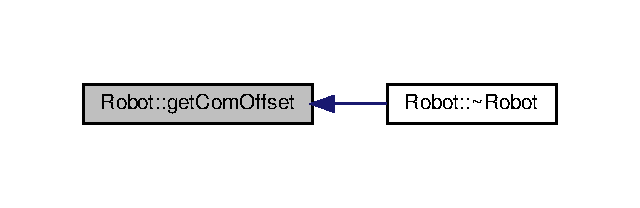
\includegraphics[width=307pt]{classRobot_a7ec7471708cfb59d26baefda819fa26b_icgraph}
\end{center}
\end{figure}
\mbox{\Hypertarget{classRobot_a3e230967bf4b167aaa20d442c6c5ceb0}\label{classRobot_a3e230967bf4b167aaa20d442c6c5ceb0}} 
\index{Robot@{Robot}!get\+Left\+Wheel\+Ang@{get\+Left\+Wheel\+Ang}}
\index{get\+Left\+Wheel\+Ang@{get\+Left\+Wheel\+Ang}!Robot@{Robot}}
\subsubsection{\texorpdfstring{get\+Left\+Wheel\+Ang()}{getLeftWheelAng()}}
{\footnotesize\ttfamily double Robot\+::get\+Left\+Wheel\+Ang (\begin{DoxyParamCaption}{ }\end{DoxyParamCaption})}



Get left steering wheel angle of robot. (in radians) 


\begin{DoxyParams}{Parameters}
{\em void} & \\
\hline
\end{DoxyParams}
\begin{DoxyReturn}{Returns}
double -\/ \hyperlink{classRobot}{Robot}\textquotesingle{}s left steering wheel angle 
\end{DoxyReturn}
Here is the caller graph for this function\+:
\nopagebreak
\begin{figure}[H]
\begin{center}
\leavevmode
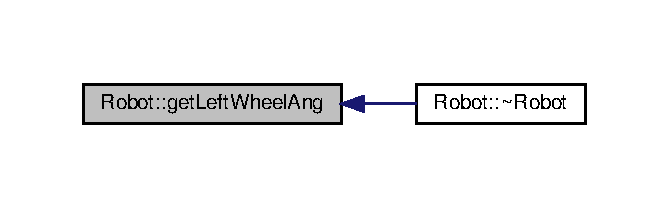
\includegraphics[width=321pt]{classRobot_a3e230967bf4b167aaa20d442c6c5ceb0_icgraph}
\end{center}
\end{figure}
\mbox{\Hypertarget{classRobot_a99559e14e93539d1deaf5f0405dfce76}\label{classRobot_a99559e14e93539d1deaf5f0405dfce76}} 
\index{Robot@{Robot}!get\+Left\+Wheel\+Vel@{get\+Left\+Wheel\+Vel}}
\index{get\+Left\+Wheel\+Vel@{get\+Left\+Wheel\+Vel}!Robot@{Robot}}
\subsubsection{\texorpdfstring{get\+Left\+Wheel\+Vel()}{getLeftWheelVel()}}
{\footnotesize\ttfamily double Robot\+::get\+Left\+Wheel\+Vel (\begin{DoxyParamCaption}{ }\end{DoxyParamCaption})}



Get left drive wheel speed of robot. (in rotations/second) 


\begin{DoxyParams}{Parameters}
{\em void} & \\
\hline
\end{DoxyParams}
\begin{DoxyReturn}{Returns}
double -\/ \hyperlink{classRobot}{Robot}\textquotesingle{}s left drive wheel speed 
\end{DoxyReturn}
Here is the caller graph for this function\+:
\nopagebreak
\begin{figure}[H]
\begin{center}
\leavevmode
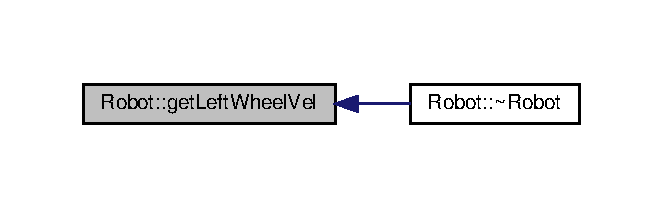
\includegraphics[width=318pt]{classRobot_a99559e14e93539d1deaf5f0405dfce76_icgraph}
\end{center}
\end{figure}
\mbox{\Hypertarget{classRobot_ad51f91ba00dfe4efa1bf0a10ea3213e6}\label{classRobot_ad51f91ba00dfe4efa1bf0a10ea3213e6}} 
\index{Robot@{Robot}!get\+Max\+Steer\+Angle@{get\+Max\+Steer\+Angle}}
\index{get\+Max\+Steer\+Angle@{get\+Max\+Steer\+Angle}!Robot@{Robot}}
\subsubsection{\texorpdfstring{get\+Max\+Steer\+Angle()}{getMaxSteerAngle()}}
{\footnotesize\ttfamily double Robot\+::get\+Max\+Steer\+Angle (\begin{DoxyParamCaption}{ }\end{DoxyParamCaption})}



Get maximum steering angle of robot. (in radians) 


\begin{DoxyParams}{Parameters}
{\em void} & \\
\hline
\end{DoxyParams}
\begin{DoxyReturn}{Returns}
double -\/ \hyperlink{classRobot}{Robot}\textquotesingle{}s max steering angle 
\end{DoxyReturn}
Here is the caller graph for this function\+:
\nopagebreak
\begin{figure}[H]
\begin{center}
\leavevmode
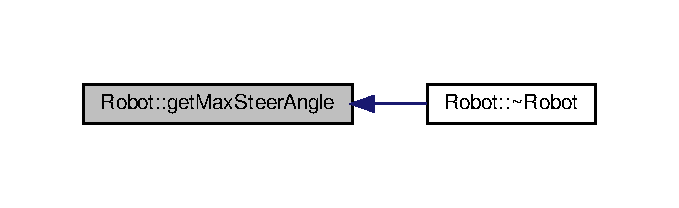
\includegraphics[width=326pt]{classRobot_ad51f91ba00dfe4efa1bf0a10ea3213e6_icgraph}
\end{center}
\end{figure}
\mbox{\Hypertarget{classRobot_aaa3dd6bad00b406b62bb58af2dd37ca4}\label{classRobot_aaa3dd6bad00b406b62bb58af2dd37ca4}} 
\index{Robot@{Robot}!get\+Right\+Wheel\+Ang@{get\+Right\+Wheel\+Ang}}
\index{get\+Right\+Wheel\+Ang@{get\+Right\+Wheel\+Ang}!Robot@{Robot}}
\subsubsection{\texorpdfstring{get\+Right\+Wheel\+Ang()}{getRightWheelAng()}}
{\footnotesize\ttfamily double Robot\+::get\+Right\+Wheel\+Ang (\begin{DoxyParamCaption}{ }\end{DoxyParamCaption})}



Get right steering wheel angle of robot. (in radians) 


\begin{DoxyParams}{Parameters}
{\em void} & \\
\hline
\end{DoxyParams}
\begin{DoxyReturn}{Returns}
double -\/ \hyperlink{classRobot}{Robot}\textquotesingle{}s right steering wheel angle 
\end{DoxyReturn}
Here is the caller graph for this function\+:
\nopagebreak
\begin{figure}[H]
\begin{center}
\leavevmode
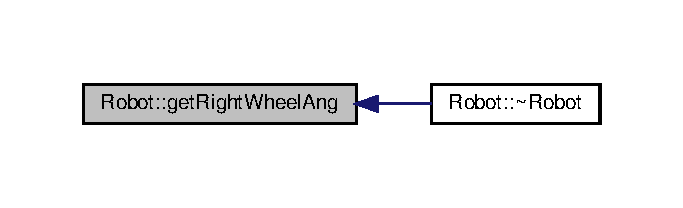
\includegraphics[width=328pt]{classRobot_aaa3dd6bad00b406b62bb58af2dd37ca4_icgraph}
\end{center}
\end{figure}
\mbox{\Hypertarget{classRobot_a4596767fd5ee2f6a923523a298d584fb}\label{classRobot_a4596767fd5ee2f6a923523a298d584fb}} 
\index{Robot@{Robot}!get\+Right\+Wheel\+Vel@{get\+Right\+Wheel\+Vel}}
\index{get\+Right\+Wheel\+Vel@{get\+Right\+Wheel\+Vel}!Robot@{Robot}}
\subsubsection{\texorpdfstring{get\+Right\+Wheel\+Vel()}{getRightWheelVel()}}
{\footnotesize\ttfamily double Robot\+::get\+Right\+Wheel\+Vel (\begin{DoxyParamCaption}{ }\end{DoxyParamCaption})}



Get right drive wheel speed of robot. (in rotations/second) 


\begin{DoxyParams}{Parameters}
{\em void} & \\
\hline
\end{DoxyParams}
\begin{DoxyReturn}{Returns}
double -\/ \hyperlink{classRobot}{Robot}\textquotesingle{}s right drive wheel speed 
\end{DoxyReturn}
Here is the caller graph for this function\+:
\nopagebreak
\begin{figure}[H]
\begin{center}
\leavevmode
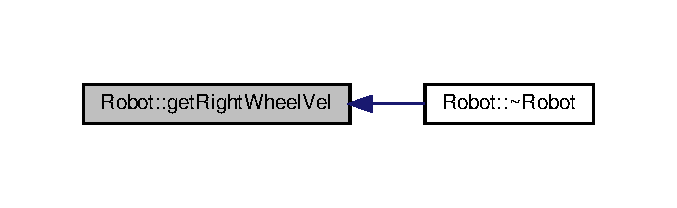
\includegraphics[width=325pt]{classRobot_a4596767fd5ee2f6a923523a298d584fb_icgraph}
\end{center}
\end{figure}
\mbox{\Hypertarget{classRobot_a4a8df828fb337ab4505f3513bd46f410}\label{classRobot_a4a8df828fb337ab4505f3513bd46f410}} 
\index{Robot@{Robot}!get\+Track\+Width@{get\+Track\+Width}}
\index{get\+Track\+Width@{get\+Track\+Width}!Robot@{Robot}}
\subsubsection{\texorpdfstring{get\+Track\+Width()}{getTrackWidth()}}
{\footnotesize\ttfamily double Robot\+::get\+Track\+Width (\begin{DoxyParamCaption}{ }\end{DoxyParamCaption})}



Get track width of robot. (in meters) 


\begin{DoxyParams}{Parameters}
{\em void} & \\
\hline
\end{DoxyParams}
\begin{DoxyReturn}{Returns}
double -\/ \hyperlink{classRobot}{Robot}\textquotesingle{}s track width 
\end{DoxyReturn}
Here is the caller graph for this function\+:
\nopagebreak
\begin{figure}[H]
\begin{center}
\leavevmode
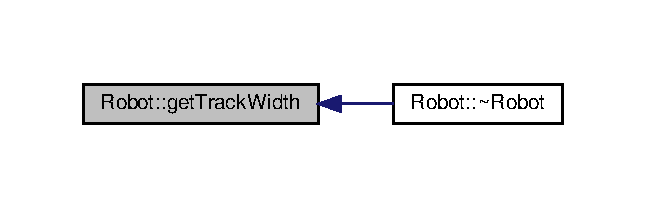
\includegraphics[width=310pt]{classRobot_a4a8df828fb337ab4505f3513bd46f410_icgraph}
\end{center}
\end{figure}
\mbox{\Hypertarget{classRobot_a31e2ab259ea221e1143141ee7765a8e2}\label{classRobot_a31e2ab259ea221e1143141ee7765a8e2}} 
\index{Robot@{Robot}!get\+Wheel\+Base@{get\+Wheel\+Base}}
\index{get\+Wheel\+Base@{get\+Wheel\+Base}!Robot@{Robot}}
\subsubsection{\texorpdfstring{get\+Wheel\+Base()}{getWheelBase()}}
{\footnotesize\ttfamily double Robot\+::get\+Wheel\+Base (\begin{DoxyParamCaption}{ }\end{DoxyParamCaption})}



Get wheelbase of robot. (in meters) 


\begin{DoxyParams}{Parameters}
{\em void} & \\
\hline
\end{DoxyParams}
\begin{DoxyReturn}{Returns}
double -\/ \hyperlink{classRobot}{Robot}\textquotesingle{}s wheel base 
\end{DoxyReturn}
Here is the caller graph for this function\+:
\nopagebreak
\begin{figure}[H]
\begin{center}
\leavevmode
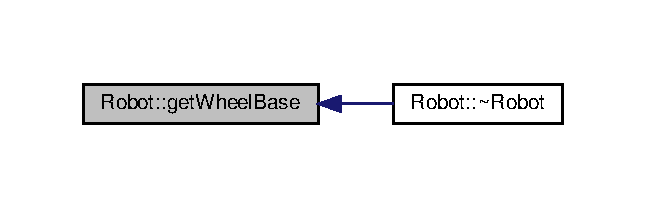
\includegraphics[width=310pt]{classRobot_a31e2ab259ea221e1143141ee7765a8e2_icgraph}
\end{center}
\end{figure}
\mbox{\Hypertarget{classRobot_a419b324c8db1f6e7e1dd65b5a15f3049}\label{classRobot_a419b324c8db1f6e7e1dd65b5a15f3049}} 
\index{Robot@{Robot}!get\+Wheel\+Radius@{get\+Wheel\+Radius}}
\index{get\+Wheel\+Radius@{get\+Wheel\+Radius}!Robot@{Robot}}
\subsubsection{\texorpdfstring{get\+Wheel\+Radius()}{getWheelRadius()}}
{\footnotesize\ttfamily double Robot\+::get\+Wheel\+Radius (\begin{DoxyParamCaption}{ }\end{DoxyParamCaption})}



Get wheel radius of robot. (in meters) 


\begin{DoxyParams}{Parameters}
{\em void} & \\
\hline
\end{DoxyParams}
\begin{DoxyReturn}{Returns}
double -\/ \hyperlink{classRobot}{Robot}\textquotesingle{}s wheel radius 
\end{DoxyReturn}
Here is the caller graph for this function\+:
\nopagebreak
\begin{figure}[H]
\begin{center}
\leavevmode
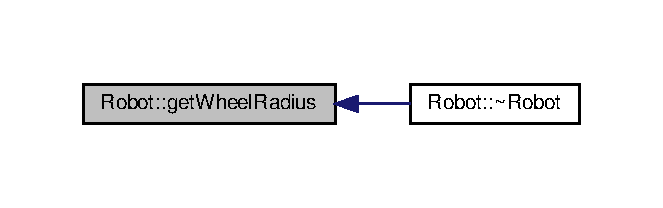
\includegraphics[width=318pt]{classRobot_a419b324c8db1f6e7e1dd65b5a15f3049_icgraph}
\end{center}
\end{figure}
\mbox{\Hypertarget{classRobot_adbe4d758d302d3fa70fedf5af9c82afc}\label{classRobot_adbe4d758d302d3fa70fedf5af9c82afc}} 
\index{Robot@{Robot}!set\+Left\+Wheel\+Ang@{set\+Left\+Wheel\+Ang}}
\index{set\+Left\+Wheel\+Ang@{set\+Left\+Wheel\+Ang}!Robot@{Robot}}
\subsubsection{\texorpdfstring{set\+Left\+Wheel\+Ang()}{setLeftWheelAng()}}
{\footnotesize\ttfamily void Robot\+::set\+Left\+Wheel\+Ang (\begin{DoxyParamCaption}\item[{double}]{ }\end{DoxyParamCaption})}



Set left drive wheel angle of robot. (in rotations/second) 


\begin{DoxyParams}{Parameters}
{\em double} & -\/ left drive wheel angle \\
\hline
\end{DoxyParams}
\begin{DoxyReturn}{Returns}
void 
\end{DoxyReturn}
Here is the caller graph for this function\+:
\nopagebreak
\begin{figure}[H]
\begin{center}
\leavevmode
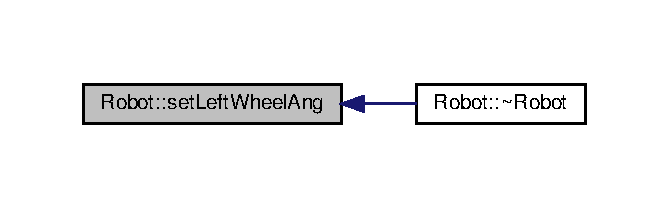
\includegraphics[width=321pt]{classRobot_adbe4d758d302d3fa70fedf5af9c82afc_icgraph}
\end{center}
\end{figure}
\mbox{\Hypertarget{classRobot_ab86642effe20a530827e4c2fc457ddb4}\label{classRobot_ab86642effe20a530827e4c2fc457ddb4}} 
\index{Robot@{Robot}!set\+Left\+Wheel\+Vel@{set\+Left\+Wheel\+Vel}}
\index{set\+Left\+Wheel\+Vel@{set\+Left\+Wheel\+Vel}!Robot@{Robot}}
\subsubsection{\texorpdfstring{set\+Left\+Wheel\+Vel()}{setLeftWheelVel()}}
{\footnotesize\ttfamily void Robot\+::set\+Left\+Wheel\+Vel (\begin{DoxyParamCaption}\item[{double}]{ }\end{DoxyParamCaption})}



Set left drive wheel speed of robot. 


\begin{DoxyParams}{Parameters}
{\em double} & -\/ left drive wheel speed \\
\hline
\end{DoxyParams}
\begin{DoxyReturn}{Returns}
void 
\end{DoxyReturn}
Here is the caller graph for this function\+:
\nopagebreak
\begin{figure}[H]
\begin{center}
\leavevmode
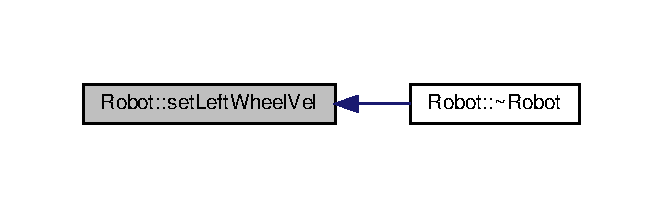
\includegraphics[width=318pt]{classRobot_ab86642effe20a530827e4c2fc457ddb4_icgraph}
\end{center}
\end{figure}
\mbox{\Hypertarget{classRobot_a3d7a12ec4cd50436d46363de93a4f9b2}\label{classRobot_a3d7a12ec4cd50436d46363de93a4f9b2}} 
\index{Robot@{Robot}!set\+Right\+Wheel\+Ang@{set\+Right\+Wheel\+Ang}}
\index{set\+Right\+Wheel\+Ang@{set\+Right\+Wheel\+Ang}!Robot@{Robot}}
\subsubsection{\texorpdfstring{set\+Right\+Wheel\+Ang()}{setRightWheelAng()}}
{\footnotesize\ttfamily void Robot\+::set\+Right\+Wheel\+Ang (\begin{DoxyParamCaption}\item[{double}]{ }\end{DoxyParamCaption})}



Set right drive wheel angle of robot. (in rotations/second) 


\begin{DoxyParams}{Parameters}
{\em double} & -\/ right drive wheel angle \\
\hline
\end{DoxyParams}
\begin{DoxyReturn}{Returns}
void 
\end{DoxyReturn}
Here is the caller graph for this function\+:
\nopagebreak
\begin{figure}[H]
\begin{center}
\leavevmode
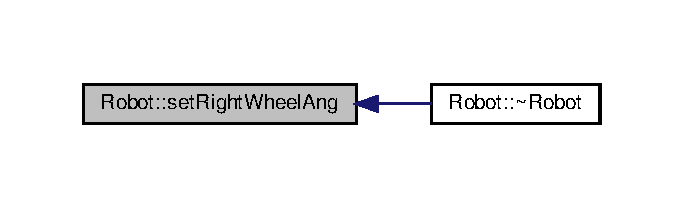
\includegraphics[width=328pt]{classRobot_a3d7a12ec4cd50436d46363de93a4f9b2_icgraph}
\end{center}
\end{figure}
\mbox{\Hypertarget{classRobot_a89e3ada15839330f45c350b67ba746f3}\label{classRobot_a89e3ada15839330f45c350b67ba746f3}} 
\index{Robot@{Robot}!set\+Right\+Wheel\+Vel@{set\+Right\+Wheel\+Vel}}
\index{set\+Right\+Wheel\+Vel@{set\+Right\+Wheel\+Vel}!Robot@{Robot}}
\subsubsection{\texorpdfstring{set\+Right\+Wheel\+Vel()}{setRightWheelVel()}}
{\footnotesize\ttfamily void Robot\+::set\+Right\+Wheel\+Vel (\begin{DoxyParamCaption}\item[{double}]{ }\end{DoxyParamCaption})}



Set right drive wheel speed of robot. 


\begin{DoxyParams}{Parameters}
{\em double} & -\/ right drive wheel speed \\
\hline
\end{DoxyParams}
\begin{DoxyReturn}{Returns}
void 
\end{DoxyReturn}
Here is the caller graph for this function\+:
\nopagebreak
\begin{figure}[H]
\begin{center}
\leavevmode
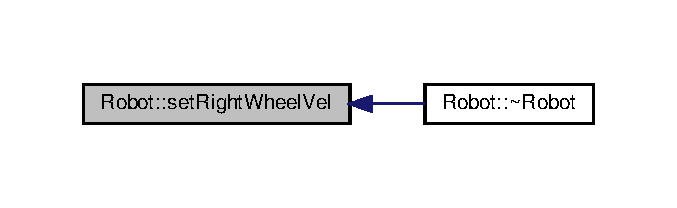
\includegraphics[width=325pt]{classRobot_a89e3ada15839330f45c350b67ba746f3_icgraph}
\end{center}
\end{figure}


The documentation for this class was generated from the following file\+:\begin{DoxyCompactItemize}
\item 
/home/maitreya/valgrind\+\_\+ws/\+Ackermann\+\_\+\+Steering\+\_\+\+Control/include/robot.\+hpp\end{DoxyCompactItemize}

\hypertarget{classSensor}{}\section{Sensor Class Reference}
\label{classSensor}\index{Sensor@{Sensor}}


Class to hold current state of robot.  




{\ttfamily \#include $<$sensor.\+hpp$>$}

\subsection*{Public Member Functions}
\begin{DoxyCompactItemize}
\item 
\mbox{\Hypertarget{classSensor_a342d6d11ef572c8cba92cb76fb1a294b}\label{classSensor_a342d6d11ef572c8cba92cb76fb1a294b}} 
\hyperlink{classSensor_a342d6d11ef572c8cba92cb76fb1a294b}{Sensor} ()
\begin{DoxyCompactList}\small\item\em Constructor for class \hyperlink{classSensor}{Sensor} to initialize robot current heading and speed to zero. \end{DoxyCompactList}\item 
\mbox{\Hypertarget{classSensor_aee8c70e7ef05ce65e7ee33686b5d7db2}\label{classSensor_aee8c70e7ef05ce65e7ee33686b5d7db2}} 
\hyperlink{classSensor_aee8c70e7ef05ce65e7ee33686b5d7db2}{$\sim$\+Sensor} ()
\begin{DoxyCompactList}\small\item\em Destructor for class \hyperlink{classSensor}{Sensor}. \end{DoxyCompactList}\item 
double \hyperlink{classSensor_a5bf3c3f5dfa3048bb702b5d3164bd410}{get\+Currernt\+Heading} ()
\begin{DoxyCompactList}\small\item\em Get current heading of robot. (in radians) \end{DoxyCompactList}\item 
double \hyperlink{classSensor_afea96ceec4830e07ed61f4ec12e45dec}{get\+Current\+Speed} ()
\begin{DoxyCompactList}\small\item\em Get current speed of robot. (in meters/second) \end{DoxyCompactList}\item 
void \hyperlink{classSensor_ade56b78666a057ce576aad448a2a5ecd}{set\+Currernt\+Heading} (double)
\begin{DoxyCompactList}\small\item\em Set current heading of robot. (in radians) \end{DoxyCompactList}\item 
void \hyperlink{classSensor_ac5cbcf17f5dc8a4d8ca545d657255f54}{set\+Currernt\+Speed} (double)
\begin{DoxyCompactList}\small\item\em Set current speed of robot. (in meters/second) \end{DoxyCompactList}\end{DoxyCompactItemize}


\subsection{Detailed Description}
Class to hold current state of robot. 

Definition at line 40 of file sensor.\+hpp.



\subsection{Member Function Documentation}
\mbox{\Hypertarget{classSensor_afea96ceec4830e07ed61f4ec12e45dec}\label{classSensor_afea96ceec4830e07ed61f4ec12e45dec}} 
\index{Sensor@{Sensor}!get\+Current\+Speed@{get\+Current\+Speed}}
\index{get\+Current\+Speed@{get\+Current\+Speed}!Sensor@{Sensor}}
\subsubsection{\texorpdfstring{get\+Current\+Speed()}{getCurrentSpeed()}}
{\footnotesize\ttfamily double Sensor\+::get\+Current\+Speed (\begin{DoxyParamCaption}{ }\end{DoxyParamCaption})}



Get current speed of robot. (in meters/second) 

\begin{DoxyReturn}{Returns}
double -\/ \hyperlink{classRobot}{Robot}\textquotesingle{}s current speed 
\end{DoxyReturn}
Here is the caller graph for this function\+:
\nopagebreak
\begin{figure}[H]
\begin{center}
\leavevmode
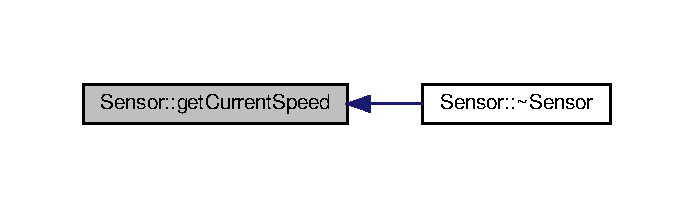
\includegraphics[width=333pt]{classSensor_afea96ceec4830e07ed61f4ec12e45dec_icgraph}
\end{center}
\end{figure}
\mbox{\Hypertarget{classSensor_a5bf3c3f5dfa3048bb702b5d3164bd410}\label{classSensor_a5bf3c3f5dfa3048bb702b5d3164bd410}} 
\index{Sensor@{Sensor}!get\+Currernt\+Heading@{get\+Currernt\+Heading}}
\index{get\+Currernt\+Heading@{get\+Currernt\+Heading}!Sensor@{Sensor}}
\subsubsection{\texorpdfstring{get\+Currernt\+Heading()}{getCurrerntHeading()}}
{\footnotesize\ttfamily double Sensor\+::get\+Currernt\+Heading (\begin{DoxyParamCaption}{ }\end{DoxyParamCaption})}



Get current heading of robot. (in radians) 


\begin{DoxyParams}{Parameters}
{\em void} & \\
\hline
\end{DoxyParams}
\begin{DoxyReturn}{Returns}
double -\/ \hyperlink{classRobot}{Robot}\textquotesingle{}s current heading 
\end{DoxyReturn}
Here is the caller graph for this function\+:
\nopagebreak
\begin{figure}[H]
\begin{center}
\leavevmode
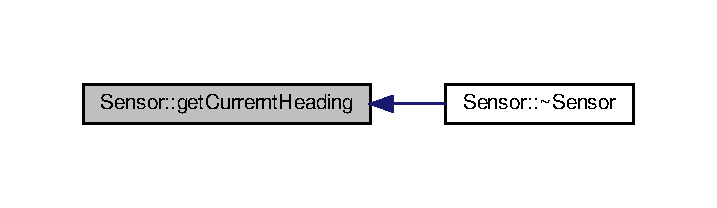
\includegraphics[width=344pt]{classSensor_a5bf3c3f5dfa3048bb702b5d3164bd410_icgraph}
\end{center}
\end{figure}
\mbox{\Hypertarget{classSensor_ade56b78666a057ce576aad448a2a5ecd}\label{classSensor_ade56b78666a057ce576aad448a2a5ecd}} 
\index{Sensor@{Sensor}!set\+Currernt\+Heading@{set\+Currernt\+Heading}}
\index{set\+Currernt\+Heading@{set\+Currernt\+Heading}!Sensor@{Sensor}}
\subsubsection{\texorpdfstring{set\+Currernt\+Heading()}{setCurrerntHeading()}}
{\footnotesize\ttfamily void Sensor\+::set\+Currernt\+Heading (\begin{DoxyParamCaption}\item[{double}]{ }\end{DoxyParamCaption})}



Set current heading of robot. (in radians) 


\begin{DoxyParams}{Parameters}
{\em double} & -\/ Current heading of robot. \\
\hline
\end{DoxyParams}
\begin{DoxyReturn}{Returns}
void 
\end{DoxyReturn}
Here is the caller graph for this function\+:
\nopagebreak
\begin{figure}[H]
\begin{center}
\leavevmode
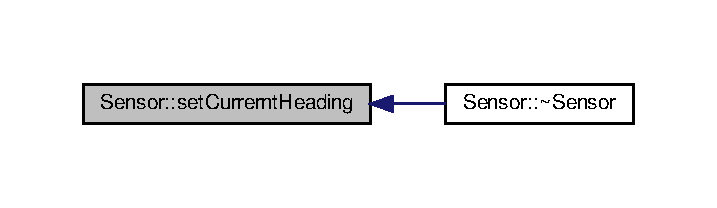
\includegraphics[width=344pt]{classSensor_ade56b78666a057ce576aad448a2a5ecd_icgraph}
\end{center}
\end{figure}
\mbox{\Hypertarget{classSensor_ac5cbcf17f5dc8a4d8ca545d657255f54}\label{classSensor_ac5cbcf17f5dc8a4d8ca545d657255f54}} 
\index{Sensor@{Sensor}!set\+Currernt\+Speed@{set\+Currernt\+Speed}}
\index{set\+Currernt\+Speed@{set\+Currernt\+Speed}!Sensor@{Sensor}}
\subsubsection{\texorpdfstring{set\+Currernt\+Speed()}{setCurrerntSpeed()}}
{\footnotesize\ttfamily void Sensor\+::set\+Currernt\+Speed (\begin{DoxyParamCaption}\item[{double}]{ }\end{DoxyParamCaption})}



Set current speed of robot. (in meters/second) 


\begin{DoxyParams}{Parameters}
{\em double} & -\/ Current speed of robot. \\
\hline
\end{DoxyParams}
\begin{DoxyReturn}{Returns}
void 
\end{DoxyReturn}
Here is the caller graph for this function\+:
\nopagebreak
\begin{figure}[H]
\begin{center}
\leavevmode
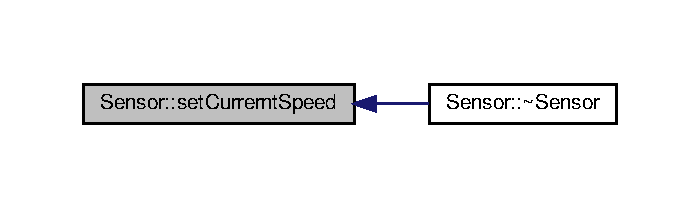
\includegraphics[width=336pt]{classSensor_ac5cbcf17f5dc8a4d8ca545d657255f54_icgraph}
\end{center}
\end{figure}


The documentation for this class was generated from the following file\+:\begin{DoxyCompactItemize}
\item 
/home/maitreya/valgrind\+\_\+ws/\+Ackermann\+\_\+\+Steering\+\_\+\+Control/include/sensor.\+hpp\end{DoxyCompactItemize}

%--- End generated contents ---

% Index
\backmatter
\newpage
\phantomsection
\clearemptydoublepage
\addcontentsline{toc}{chapter}{Index}
\printindex

\end{document}
